
\chapter{图像检索及几何校验基础}
在本章中,将首先介绍基于BoW和CNN的图像检索框架,然后基于这些检索框架,介绍主流的空间校验算法,包括检索后校验和检索时校验。随后,还介绍了近年来的一些最新工作和研究趋势,并以此为基础,确定了本文的研究思路和框架。

\section{基于BoW的检索框架}
基于内容的图像检索(Content Based Image Retrieval)是在给定查询图像的前提下,依据内容信息或指定查询标准,在图像数据库中搜索并找出符合查询条件的相应图片\cite{cyy2007img}。 
随着网络以及多媒体技术的迅速发展,数字图像的数量正在不断迅速的增长,对数字图像的自动化管理与检索,也成为新时代迫切的需求。然而,传统的基于关键字检索的方式,需要人工对图像内容进行标注,不仅工作量巨大,同时也存在人工标注的文字歧义等问题。在这样的背景下,基于内容的图像检索技术应运而生。
最早的基于内容的图像检索应用成功的是IBM开发的QBIC\cite{qbic}(Query By Image Content)系统,通过用户指定按例子查询或者按绘制草图查询,它利用了颜色、纹理、形状等特征对图像进行分析,从而查找出符合用户意图的图像。
由于基于内容的图像检索技术从图像内容本身出发,无需人工干预或者主动标记,大大减轻了多媒体管理人员的负担,因而被广泛的应用于电子图书馆、医学分析、博物馆等领域;与此同时,基于内容的图像检索也常常用于网购、拷贝检测等大众产品之中。
在大规模图像检索系统中,词袋模型(BoW)是目前为止最为成功的模型之一\cite{arandjelovic2012three},相比其它模型(如VLAD\cite{jegou2010aggregating}, FisherVector\cite{perronnin2007fisher}),BoW具有易于实现,扩展众多的优点,非常利于工程化实现调优。图\ref{fig:bow}形象的描绘了BoW模型的思想。

\subsection{Hessian Affine区域及SIFT描述子}
在基于BoW的检索框架中,最核心的部分是如何在图像中提取类似于文本中的“单词”的特征,在CBIR中称为视觉单词(Visual Word)。在得到视觉单词之前,首先要提取图片的局部特征。提取局部特征的经典方法是首先在图片中寻找Hessian Affine区域\cite{mikolajczyk2004scale},然后在该区域上提取SIFT\cite{lowe2004distinctive}描述子。其中Hessian Affine区域保证了仿射不变性,而SIFT描述子保证了旋转和尺度不变性。SIFT描述子具有以下特征:
\begin{enumerate}
	\item SIFT特征是图像的局部特征,对旋转、尺度缩放、亮度变化等均具有不变形,对视角变化、仿射变换、噪声也具有一定程度的稳定性;
	\item 独特性好,信息量丰富,适于在海量特征数据库中进行快速、准确的匹配;
	\item 多量性,即使少数的几个物体也可以产生大量的SIFT特征向量;
	\item 高速型,经优化的SIFT匹配算法甚至可以达到实时的要求;
	\item 可扩展性,可以很方便的与其他形式的特征向量进行联合;
\end{enumerate}

正是因为SIFT具有以上特性,BoW模型通常都选用SIFT对图像局部特征进行描述。SIFT特征检测主要包括以下四个基本步骤:
\begin{enumerate}
	\item 尺度空间极值检测:搜索所有尺度上的图像位置,通过高斯微分函数来识别潜在的对于尺度和旋转具有不变性的兴趣点。
	\item 关键点定位:在每个候选位置上,通过一个拟合精细的模型来确定位置和尺度,依据候选点的稳定程度选取关键点。
	\item 方向确定: 基于图像局部的梯度方向,分配给每个关键点位置一个或多个方向,后面对关键点的特征描述都相对于关键点的方向,尺度和位置进行变化,从而保证特征描述的不变性。
	\item 关键点描述:在每个关键点周围的领域内,根据所选尺度,在图像局部计算梯度直方图,并连接为一个128维的向量。
\end{enumerate}

\subsection{建立视觉词典}
在提取局部特征之后,特征还没有转化为视觉单词。就像在文本检索中,无论哪种语言都会有一个词典,在BoW图像检索框架中仍然需要建立词典(区别于文本词典,这里成为视觉词典)。构建视觉词典的一般方法是:首先提取大量的局部特征(描述符),一般是视觉单词数的十倍以上;然后使用K-Means方法进行聚类;最后所有的聚类中心即为视觉词典。假设要形成k个视觉单词,K-Means算法描述如下:
\begin{enumerate}
	\item 适当选择k个类的初始中心;
	\item 在第i次迭代中,对任意一个样本,求其到k个中心的距离,将该样本归到距离最短的中心所在的类;
	\item 利用均值等方法更新该类的中心值;
	\item 对于所有的k个聚类中心,如果重复利用2,3步骤进行迭代更新后,值保持不变(或者指定一个变化阈值),则迭代结束,否则继续迭代。
\end{enumerate}

在实际操作中,通常在另外一个数据集上提取特征并建立视觉字典。根据检索任务的不同,视觉字典的大小也不同,一般会选取几千至几百万之间。由于K-Means算法时间复杂度高,尤其是当聚类中心比较多的时候,现在主流的方法是使用Approximate K-Means(AKM)\cite{philbin2007object}。

\subsection{TF-IDF权重}
通过建立视觉词典,我们可以把一张图片表示为一个BoW向量,向量的长度与字典大小相同。假设图片$I$的BoW向量为$T=[t_1,t_2,...,t_k]$,其中$k$为字典中包含的视觉单词数。此时,$T(i)=t_i$表示在图片$I$中包含视觉单词$i$的个数。

在文本检索中,每个文档用词频向量来表示,基于BoW的图像检索框架就是借鉴了文本检索的表示方式。在文本检索中最常用的加权方案是“词频-逆文档频率”加权,表示为$tf\_idf$。$tf\_idf$的计算方式如下:
\begin{equation}
tf\_idf_i=\frac{n_{id}}{n_d}\log\frac{N}{n_i}
\end{equation}
其中,$n_{id}$是在文档$d$中出现单词$i$的次数,$n_d$是文档$d$包含的单词总数,$n_i$是单词$i$在整个数据库中出现的次数,$N$是数据库中文档数。这种加权方式由两部分的乘积组成,分别是词频(word frequency)$tf$和逆文档频率(inverse document frequency)$idf$。$tf$表示了一个单词在一篇文档中的重要程度,而$idf$表示了这个单词在整个文档库中的重要程度。使用$tf\_idf$加权模型后,一副图像的BoW向量表示为$T=[tf\_idf_1,tf\_idf_2,...,tf\_idf_k]$

\subsection{建立倒排索引}
在线实际检索时,由于通常图像库很大(例如百万级别),此时如果通过线性比较计算图像之间的相似性,速度是不可忍受的,为此需要建立某种形式的索引,以提高检索效率。通常采用倒排索引。
\begin{figure}[h]
	\centering
	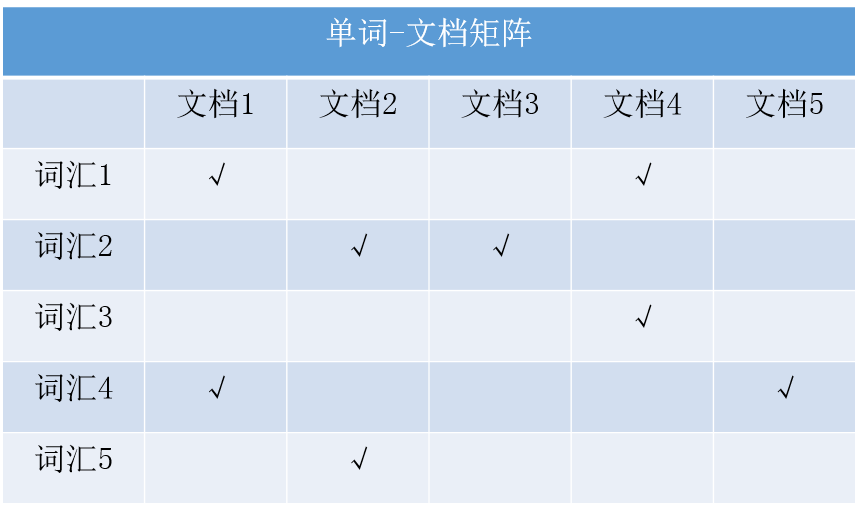
\includegraphics[width=0.8\textwidth]{invindex.png}
	\caption{倒排索引示例}\label{fig:invindex}
\end{figure}
如图\ref{fig:invindex}所示为一个单词-文档矩阵,其中打勾则代表包含关系。从纵向即文档的维度来看,每列代表文档包含了哪些单词,即正向索引。而横向即从单词的维度来看,每行代表了哪些文档包含了某个单词。倒排索引即从单词的维度来看,建立的单词-文档矩阵。如此建立索引后,每次在线查询时,只需要将得到的局部特征映射为视觉单词,然后通过倒排索引的单词-文档矩阵,就可以查找到所有包含该单词的文档,最后通过tf-idf进行评分,即可将相关的文档进行评分。倒排索引高效的关键在于,每个文档包含的视觉单词只是整个视觉字典中很小的一部分,即单词-文档矩阵是稀疏的,这样在检索时,只需要计算BoW向量和倒排索引中的非0部分,大大提高了检索的效率。

\subsection{整体系统框架}
\begin{figure}[h]
	\centering
	\includegraphics[width=\textwidth]{Bow_frame.jpg}
	\caption{BOW模型框架图}\label{fig:bowframe}
\end{figure}
整体框架如图\ref{fig:bowframe}所示,离线训练时,我们从一组图像集合中提取局部特征,然后对其进行聚类,我们将聚类中心作为视觉单词,形成视觉词典。在线检索时,我们首先提取图像的局部点特征(SIFT),然后将每一个点特征进行量化(查找与视觉词典中的视觉单词欧氏距离最近的单词),形成词频向量,最后通过倒排索引,对相关图像进行评分,排序后,输出相似图像。

\section{一些对BoW的改进方案}
在基于BoW的图像检索框架提出之后的十几年里,有许多改进方案\cite{philbin2007object}\cite{philbin2008lost}\cite{chum2007total}\cite{jegou2008hamming}\cite{turcot2009better}
\cite{zheng2014bayes}\cite{zheng2014packing}\cite{knopp2010asvoiding}\cite{zhou2011large}被提出来提高检索的准确率或召回率。除了几何校验(geometric verification)之外,还包括查询扩充(query expansion)\cite{chum2007total}\cite{shen2012Object}、软分配(soft assignment)\cite{philbin2008lost}、特征注入技术(embedding)\cite{jegou2008hamming}\cite{jegou2014triangulation}、burstness\cite{jegou2009burstiness}\cite{shi2015early}、和对SIFT特征的修改(RootSIFT)\cite{arandjelovic2012three}等等。本章将对文本实验中使用到的一些改进方案做基本的介绍,下一章将对几何校验的方法做详细介绍。

\subsection{查询扩充}
本节主要介绍\cite{chum2007total}和\cite{shen2012Object}中提出的查询扩充的思想和方法。Query Expansion(QE)的思想为根据第一次检索得到的结果再进行一次或多次检索,并将多次检索的结果融合得到最终的检索结果。

\cite{chum2007total}提出了多种QE方案,其中最为常用的是平均QE(Average Query Expansion,AQE)。在AQE中,对原始查询的结果(BoW向量)取均值来构建一个新的查询。首先,查询系统得到原始查询的$m$个结果($m$一般小于50,并且结果是经过空间校验的);通过求原始查询和$m$个原始查询的平均值得到一个新的查询$Q_{avg}$:
\begin{equation}
d_{avg}= \frac{1}{m+1}(d_0+\sum_{i=1}^{m}d_i)
\end{equation}
其中$d_0$是原始查询的BoW向量(归一化的词频向量),$d_i$是原始查询检索到的第$i$个结果。接下来使用$Q_{avg}$进行新一轮的检索,并将检索结果插入到原始结果的第$m$之后。

可以看出在AQE中,查询结果与原始查询是被同等对待的,并且也没有考虑查询结果出现的位置关系。\cite{shen2012Object}对\cite{chum2007total}提出的AQE进行了改进,提出了k-NN re-ranking(k-NNQE)。令$S$表示查询图片和数据库图片的相似度,则根据$S$可以得到数据库图片的排序$R(Q,D)$,其中$Q$为查询图片,$D$为数据库图片。令$N_i$为查询结果的第$i$个图片,则$R(Q,N_i)=i$,并且$\mathcal{N}_q=\{N_i\}_\{i=1,...,k\}$为查询的$k$近邻。图\ref{fig:k-NNQE}解释了k-NNQE算法,数据库图片的得分由它在原始查询中的排序和k-NN中的排序共同决定。
\begin{figure}[h]
	\centering
	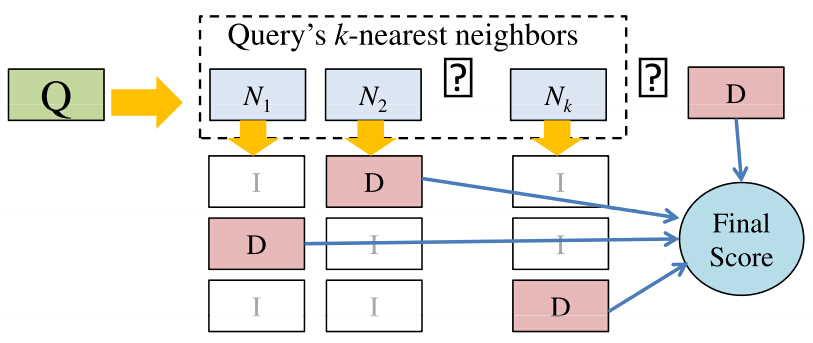
\includegraphics[width=0.7\textwidth]{k-NNQE.jpg}
	\caption{k-NNQE}\label{fig:k-NNQE}
\end{figure}
在k-NNQE中一张数据库图片$D$的得分有两部分组成,包括$D$在原始查询结果中的位置和在$k$近邻作为查询的结果中的位置。令$D$在$N_i$查询结果中的排序为$R(N_i,D)$,则$D$的最终得分为:
\begin{equation}
\bar{S}(Q,D)=\frac{w_0}{R(Q,D)}+\sum_{i=1}^{k}\frac{w_i}{R(N_i,D)}
\end{equation}
其中$w$为权重。由于最近邻的排序不同,其权重也应该不同,所以设置$w_0=1$,$w_i=1/(R(Q,N_i)+1)=1/(i+1)$。查询本身可以认为是$N_0$,所以$D$的最终得分表示为:
\begin{equation}
\bar{S}(Q,D)=\sum_{i=0}^{k}\frac{w_i}{R(N_i,D)}=\sum_{i=0}^{k}\frac{1}{(i+1)R(N_i,D)}
\end{equation}
图\ref{fig:k-NNQE_exa}展示了k-NNQE算法在Oxford数据集上\cite{philbin2007object}的一个实例。相比于AQE的方法,k-NNQE在重排序中考虑了查询结果的相对位置关系,并且对outliers不敏感,这使得k-NNQE会得到更高的准确率。但是,由于k-NNQE需要对每个$k$近邻都进行重新检索,效率很低。无论是AQE还是k-NNQE都可以递归进行多次来提高检索效果。
\begin{figure}[h]
	\centering
	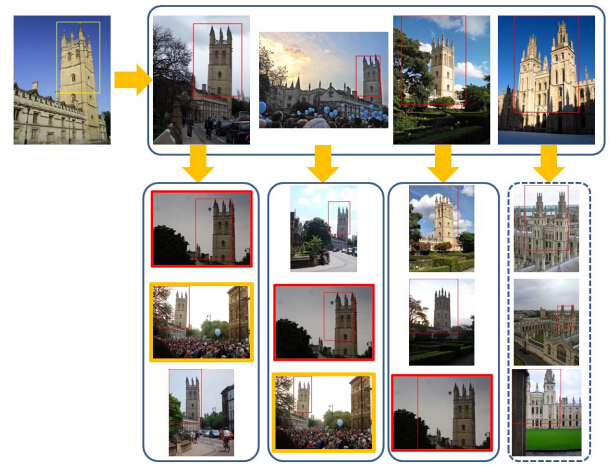
\includegraphics[width=\textwidth]{k-NNQE_exa.jpg}
	\caption{k-NNQE算法实例}\label{fig:k-NNQE_exa}
\end{figure}

\subsection{软分配}
软分配(Soft Assignment,SA)又称为软量化,是缓和BoW检索框架中量化误差的一种解决方案,本节主要介绍\cite{philbin2008lost}中提出的SA算法。

在原始的BoW检索框架中,每个描述符要量化到一个视觉单词,之后每个描述符就用视觉单词来表示,这样会大大减少特征空间,但是不可避免的引入了量化误差。图\ref{fig:sa}描述了一般量化的缺点,在图中,点A到E表示视觉单词(k-Means聚类中心),1到4为特征描述符,点1、2、3将被量化到视觉单词A,点4将被量化到视觉单词C,这导致实际上很相似的两个点3和4永远无法匹配,SA就是用来解决这个问题。
\begin{figure}
	\centering
	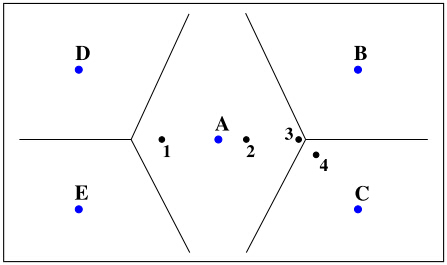
\includegraphics[width=0.7\textwidth]{soft_assignment.jpg}
	\caption{软量化的优点}\label{fig:sa}
\end{figure}
在\cite{philbin2008lost}中,量化时不是将某个描述符只分配到离它最近的聚类中心(视觉单词),而是分配给若干个聚类中心。分配的权重与描述符到中心的距离成反比,具体表示为:
\begin{equation}
w=exp(-\frac{d^2}{2\rho^2})
\end{equation}
其中$d$表示描述符到中心的距离,$\rho$控制权重,同时会设置参数$r$,表示最多分配给多少个聚类中心。当分配给多个中心后,将权重进行L1归一化。通过软量化,可以一定程度上解决量化误差的问题。例如,在图\ref{fig:sa}中,假设$r=3$,这时点3和4将分配给中心A、B和C,这样描述符3和4就可以以很高的相似度匹配。而点1将分配给A、D和E,所以描述符1和3就不会得到较高的匹配得分。可以看出,由于每个描述符分配给$r$个聚类中心,所以倒排表的大小大约为硬量化的$r$倍,并且软量化也会导致查询速度下降。

在\cite{jegou2009burstiness}中提出了SA的简化版本,即不考虑描述符到聚类中心的距离,以相同的权重分配给最近的$r$个中心,这种方法被称为多分配(Multi-Assignment,MA)。\cite{jegou2009burstiness}中只对查询图片进行了MA,而没有对数据库图片进行MA,所以只是增加了检索时间,而没有增加内存消耗。

\subsection{注入技术}
在选择视觉词典的大小时(聚类中心的个数),有一个两难的问题,即选择聚类中心数$k$是量化噪声(Quantization Noise)和描述符噪声(Descriptor Noise)之间的取舍\cite{jegou2008hamming}。
\begin{figure}[h]
	\centering
	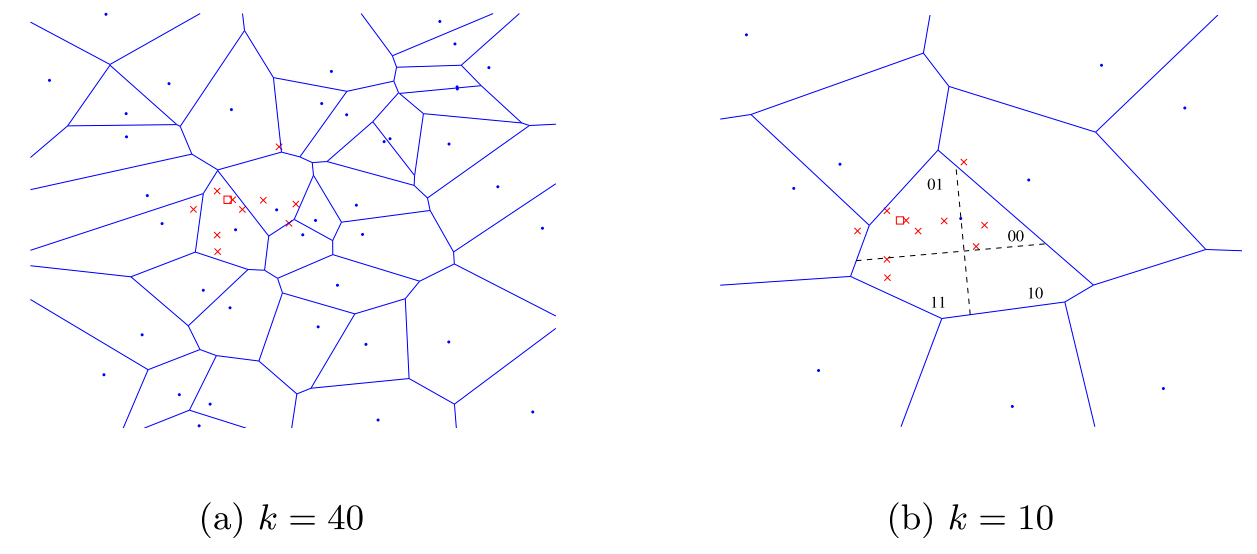
\includegraphics[width=\textwidth]{centroids.jpg}
	\caption{不同聚类中心数的K-Means聚类,以及Hamming Embedding方法}\label{fig:centroids}
\end{figure}
图\ref{fig:centroids}解释了这个两难的问题,其中$k$表示聚类中心数。当聚类中心较多时((a)情况),一个有噪声的描述符将被分配到不同的聚类中心,此时描述符噪声对检索结果影响很大;当聚类中心较少时((b)情况),不相似的描述符可能被分配到同一个聚类中心,此时量化噪声较大。\cite{jegou2008hamming}和\cite{jegou2014triangulation}采用注入技术(Embedding)来解决这个问题。本节重点介绍Hamming Embedding技术\cite{jegou2008hamming}。

Hamming Embedding结合了低聚类中心高召回率和多聚类中心高准确率的特点。其思想是为每个描述符分配一个二进制串来表示其在Voronoi区域中的位置。如\ref{fig:centroids}(b)所示,中间的Voronoi区域被分成了若干个子区域。令$x$和$y$为两个描述符,他们的二进制串为$b(x)$和$b(y)$。则需要设计一种二进制串,使他们的海明距离:
\begin{equation}
h(b(x),b(y))=\sum_{i}^{}1-\theta_{b(x),b(y)}
\end{equation}
可以反映出$x$和$y$在同一个Voronoi区域中的距离。\cite{jegou2008hamming}提出了一种基于学习的方案来实现Hamming Embedding,分为离线(offline)操作和在线(online)操作两部分。

Offline操作:
\begin{enumerate}
	\item 生成随机投影矩阵$P$:生成一个$d_b \times d$的随机正交矩阵,其中$d_b$为二进制串的长度,$d$为描述符的长度(例如SIFT描述符$d=128$)。首先生成一个$d \times d$维随机高斯矩阵,然后对该矩阵进行QR分解,取正交矩阵的前$d_b$行作为投影矩阵$P$;
	\item 描述符的投影和分配:首先在一个独立的数据库上提取一个描述符集合,然后对每个描述符$x$进行量化($q(x)$)和投影操作($Px$);
	\item 计算投影的描述符的中值:每个聚类中心对应有一个投影的描述符集合,求出这些描述符的中值,即对应每一维上的中值组成的新向量。
\end{enumerate}

经过上述操作,我们可以在线下得到一个投影矩阵$P$和视觉词典的每个聚类中心(即视觉单词)的中值向量$m$。

Online操作:
\begin{enumerate}
	\item 分配:对于一个描述符,将该描述符分配给距离它最近的视觉单词$q(x)$;
	\item 投影:使用投影矩阵$P$对$x$进行投影,得到$z=Px=(z_1,...,z_{d_b})$;
	\item 计算二进制串$b(x)=(b_1(x),...,b_{d_b(x)})$:
	\begin{equation}
	b_i(x)=
	\begin{cases}
	1& \text{if $z_i > m_{q(x),i}$}\\
	0& \text{otherwise}
	\end{cases}
	\end{equation}
\end{enumerate}

经过上述操作,每个描述符$x$由$q(x)$和$b(x)$表示。则在Hamming Embedding的条件下,两个描述符的匹配表示为:
\begin{equation}
f_{HE}(x,y)=
\begin{cases}
tf\_idf(q(x))& \text{if $q(x)=q(y)$ and $h(b(x),b(y)) \le h_t$}\\
0& \text{otherwise}
\end{cases}
\end{equation}

在实际检索中,一般$d_b = 64$,$22 \le h_t \le 24$。由于Hamming Embedding减少了检索过程中的误匹配,所以会大大提高检索的精度。但是Hamming Embedding并不适合大字典的情况(一般字典长度为20k到200k之间),并且由于每个描述符要注入一个二进制串,需要额外的内存开销。

\subsection{RootSIFT}
在BoW检索框架中,其基本原理是通过计算SIFT描述符之间的相似度(余弦距离或欧式距离)来计算图片的得分。而实际上,使用Hellinger距离计算相似度会得到更好的结果。\cite{arandjelovic2012three}提出RootSIFT,使得在传统的BoW框架下可以使用Hellinger距离度量SIFT描述符之间的相似度。

令$x$和$y$为两个描述符,并且$\parallel x \parallel^2_2 = \parallel y \parallel^2_2 = 1$,则他们的欧式距离$d_E(x,y)^2$和欧式相似核$S_E(x,y)$的定义如下:
\begin{equation}
d_E(x,y)^2 = \parallel x-y \parallel^2 = \parallel x \parallel^2_2 + \parallel y \parallel^2_2 - 2x^Ty = 2 - 2S_E(x,y)
\end{equation}
\cite{arandjelovic2012three}将欧式相似核$S_E(x,y)$替换为Hellinger核。假设$x$和$y$是L1归一化的,则Hellinger核的定义为:
\begin{equation}
H(x,y) = \sum_{i=1}^{n}\sqrt{x_iy_i}
\end{equation}
SIFT描述符可以通过两个简单的步骤转化为RootSIFT:
\begin{enumerate}
	\item L1归一化SIFT描述符;
	\item 对L1归一化的SIFT描述符的每一维开方。
\end{enumerate}

经过上述变换后的描述符被称为RootSIFT,计算RootSIFT描述符之间的欧式距离相当于计算SIFT描述符之间的Hellinger距离(具体证明参见\cite{arandjelovic2012three})。RootSIFT不会增加计算复杂和内存消耗,并且几乎可以与任何现有的基于SIFT的检索框架融合,已经成为BoW检索中的基本处理步骤。

\section{基于CNN的检索框架}
在计算机视觉领域,卷积神经网络(Convolutional Neural Network,CNN)得到了广泛的应用\cite{zhang2015bit}\cite{hu2014discriminative}\cite{schroff2015facenet}\cite{hariharan2015hypercolumns}\cite{papandreou2015modeling}\cite{yuting2015improving}\cite{lenc2014understanding}\cite{nguyen2014deep}。LeNet\cite{lecun1998Gradient}在手写数字识别上达到了99\%以上的准确率。AlexNet\cite{krizhevsky2012imagenet}在ImageNet LSVRC-2010和ILSVRC-2012得到了同年最好的结果,相比于传统方法得到了质的提升,而\cite{he2015delving}在ILSVRC-2012上甚至得到比人更高的分类准确率。除了分类问题,CNN在目标检测\cite{Girshick2014Rich}\cite{girshick2015fast}\cite{ren2015faster}、人脸识别等计算机视觉领域同样取得了突破。2014年\cite{babenko2014neural}将CNN应用到图像检索领域,由于CNN相比基于BoW的方法,可以更好的提取图片的语义信息,因此\cite{babenko2014neural}取得了很好的检索效果。下面就对\cite{babenko2014neural}中的检索框架进行介绍。

\begin{figure}[h]
	\centering
	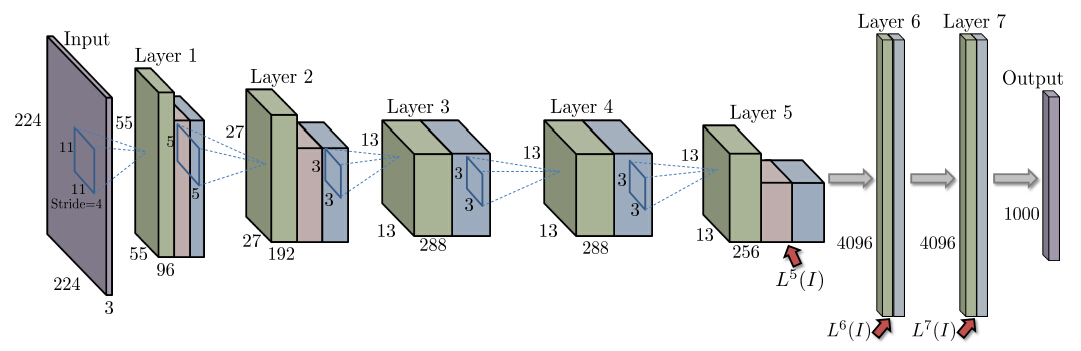
\includegraphics[width=\textwidth]{AlexNet.jpg}
	\caption{AlexNet网络结构}\label{fig:AlexNet}
\end{figure}

\cite{babenko2014neural}提出的检索框架主要基于AlexNet。图\ref{fig:AlexNet}展示了AlexNet\cite{krizhevsky2012imagenet}的网络结构。在该网络中除了第一层的输入层(input)和最后一层的输出层(output),前5层为卷积网络(表示为conv),每层卷积网络后会跟随激活层(一般使用rectified linear transform,表示为relu)和Pooling层(表示为pool)。网络的第6层和第7层为全连接层(表示为fc),一般每个全连接层后会跟随激活层和DropOut层(表示为dropout)。

则基于CNN的检索过程如下:
\begin{enumerate}
	\item 训练CNN网络:一般是使用在ImageNet上已经训练好的CNN网络,这主要是由于目前还没有图像检索的大规模数据库;
	\item *fine-tune:使用检索数据集或相似数据集对CNN网络进行再训练,即初始化参数使用ImageNet训练的网络的参数;
	\item 特征提取:向训练好的网络(或经过fine-tune)输入需要提取特征的图片,并将网络中某些层的输出作为该图片的特征;
	\item *后处理:一般可以使用PCA对提取的特征进行降维;
	\item 建立特征库并进行检索。
\end{enumerate}

其中标*的部分为非必须操作。提取图片特征时,一般会选择全连接层的输出或最后一个Pooling层的输出作为特征,在图\ref{fig:AlexNet}中就是第5、6、7层,表示为$L^5(I)$、$L^6(I)$、$L^7(I)$,其中$I$表示图片。可以看出,不同于BoW检索框架中使用局部特征(如SIFT),CNN提取的特征是全局特征(即每张图片一个特征)。

可以看出基于CNN的图像检索框架要比基于BoW的检索框架简单,其原因可能是基于CNN的检索框架刚提出不久,很多问题和解决办法还没有被提出来;另一方面也是因为CNN网络自身具有较强的能力(几百万到上亿的参数量)。但是目前基于CNN的检索框架并没有解决一般图像检索中普遍存在的问题,如旋转等。本文将在这方面对其作出改进。


\section{主流的几何校验算法}
自基于BoW的图像检索框架提出以来(包括\cite{sivic2003video}),人们对几何校验的研究一直没有中断。这是因为BoW检索框架中忽略了视觉单词之间的几何信息,而加入几何校验之后会显著提高BoW检索的精度。本节将介绍几种经典的几何校验方案,包括Fast Spatial Matching(FSM)\cite{philbin2007object}、Weak Geometric Consistency(WGC)\cite{jegou2008hamming}和Spatial Pyramid Matching(SPM)\cite{lazebnik2006beyond}。这些方法也是其他几何校验方法的基础。

\subsection{Fast Spatial Matching}
FSM\cite{philbin2007object}的核心思想是通过一对匹配的特征点来确定图片的之间的仿射变换矩阵,然后去验证其他点对是否满足这个变换。FSM中有一个关键假设就是重力向量假设\cite{perd2009efficient},即所有特征的主方向是垂直的,也就是说图片必须是垂直的。
\begin{figure}[h]
	\centering
	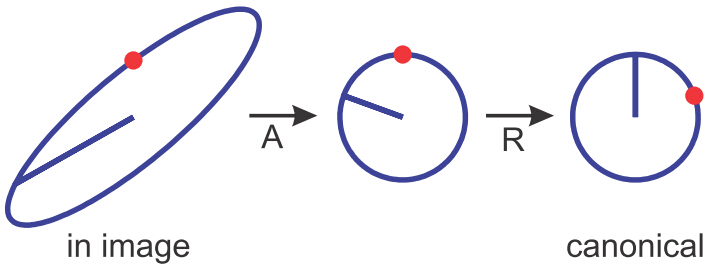
\includegraphics[width=0.6\textwidth]{ellipse.jpg}
	\caption{一个SIFT描述符的椭圆几何空间}\label{fig:ellipse}
\end{figure}


对于每个SIFT特征,除了其描述符信息,还包含几何信息(一般表示为一个椭圆,如图\ref{fig:ellipse},其中$A$为映射矩阵,$R$为旋转矩阵)。对于一个有椭圆空间信息的特征点$u$,它满足如下等式:
\begin{equation}
(u-u_0)^TE(u-u_0)=1
\end{equation}
其中$u_0$是椭圆的中心,$E\in \mathbb{R}^{2 \time 2}$是一个正定矩阵。在这个椭圆上的点(如图\ref{fig:ellipse}中的红点)可以通过一个映射矩阵$A\in\mathbb{R}^{2 \time 2}$映射到一个单位圆上面,其中$E=A^TA$,并且椭圆的尺度为$\frac{1}{det A}$。如果$A$是一个下三角矩阵,则相应的仿射变换有一个为$[0 ~1]^T$的特征值。

对于一个匹配的特征对$\{x_q,x_g\}$,通过分解他们的椭圆矩阵$E_q$和$E_g$,可以得到下三角映射矩阵$A_q$和$A_g$。令$R_q$和$R_g$为对点的旋转矩阵,$M_s$描述这对点的尺度和旋转变换,则有:
\begin{equation}
M_s=A_g^{-1}R_g^TR_qA_q
\end{equation}
由于DSM要求特征满足重力向量假设,则要求$R_g^TR_q=I$\cite{perd2009efficient},所以$M_s=A_gA_q$。因此,变换向量可以写为:
\begin{equation}
t=x_g-M_sx_q
\end{equation}

当$t$的L2模小于某个阈值时,则认为这对点对是具有几何一致性的(inliers)。在FSM中,需要根据每个匹配的点对算出一个可能的变换矩阵$M_s$,并用这个$M_s$去验证其余的点对。当找到使inliers最多的变换矩阵时,就认为该变换矩阵为这对图片的变换矩阵。可以通过设定阈值,当inliers小于该阈值时,认为两张图片不匹配,或根据inliers数对图片进行打分来进行几何校验。

由于FSM需要对每个匹配点对计算一个变换矩阵,并用该矩阵测试其他点对,所以FSM的时间复杂度为$O(n^2)$。在实际的检索中,FSM只作为检索后校验算法,一般会对Top100到Top800的检索结果进行几何校验。

\subsection{Weak Geometric Consistency}
由于FSM的高时间复杂度,\cite{jegou2008hamming}提出了一种弱几何校验方案WGC,WGC只考虑特征点对之间的尺度和角度的差值。所以在WGC中,每个SIFT特征的几何关系不是用一个椭圆来表示,而只用角度(angle)和尺度(scale)来表示。其中角度编码了特征区域的梯度方向,而尺度编码了特征区域的范围。

对于一张图片$j$,$s_j$表示由尺度和角度差值组成的二维直方图。其中每个cell表示为$s_j(\delta_a,\delta_s)$。其中$\delta_a$和$\delta_s$分别表示匹配的特征区域间的量化的角度(angle)和对数尺度(log-scale)差。通过$s_j$,图像的几何校验得分可以表示为:
\begin{equation}
s_j^*=g( \max \limits_{(\delta_a,\delta_s)} s_j(\delta_a,\delta_s) )
\end{equation}

在实际的计算中,angle和scale的分布是具有很强独立性的,所以没有必要将这两个值量化到同一个直方图内,可以将他们分别量化到两个一维的直方图,$s_j^a(\delta_a)$和$s_j^s(\delta_s)$。在这种情况下,图片的得分可以表示为:
\begin{equation}
s_j^*=g( \min (\max \limits_{\delta_a}(\delta_a), \max \limits_{\delta_s}(\delta_s)) )
\end{equation}

可以看出WGC也是一种后校验方案,即只对匹配的特征点进行校验。为了加快检索速度,WGC会将角度和尺度信息编码到倒排表中,带来一部分的内存开销。同时,WGC无法解决图片旋转的问题,在实际检索中,一般假设图片只可能有四个方向(即0度、90度、180度和270度),并在WGC中的$\delta_a$相应的cell上增加权重。

\subsection{Spatial Pyramid Matching}
前面两节介绍了两种经典的后校验算法,由于后检验一般速度较慢,且只能对匹配的点对进行校验,这里介绍一种经典的检索时校验方案,Spatial Pyramid Matching(SPM)\cite{lazebnik2006beyond}。
\begin{figure}[h]
	\centering
	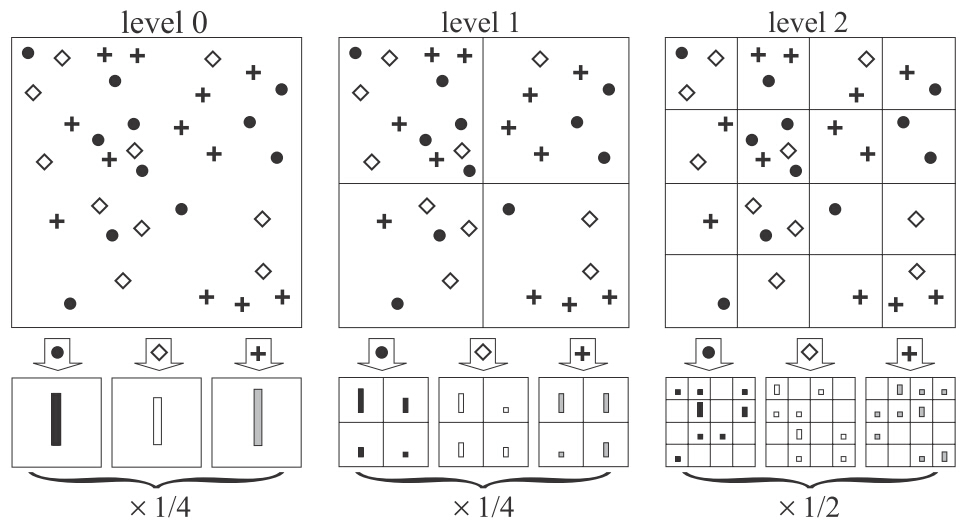
\includegraphics[width=0.8\textwidth]{SPM.jpg}
	\caption{Spatial Pyramid Matching示意图}\label{fig:SPM}
\end{figure}

SPM的核心思想是将图片划分为若干不同尺度的区域,对每个区域构建一个BoW向量,最后将所有这些BoW向量连接起来作为图像的BoW向量。在检索时,只有对应区域的BoW向量可以匹配,所以可以保证一定的空间一直性。图\ref{fig:SPM}描述了将一张图片按水平和垂直方向分为进行三个尺度划分的情况。可以看出当划分的粒度越细时,具有越强的空间校验。

在进行匹配时,SPM使用Spatial Pyramid核计算相似度。假设有图片$X$和$Y$,我们将图片在$0,...,L$个分辨率上进行分割,图\ref{fig:SPM}表示了$L=2$的情况。在分辨率$l$上,图片的每个维度被分割成$2^l$份,在所有维度$d$上,图片一共会被分成$D=2^{dl}$个子区域。假设在$l$分辨率上,$X$和$Y$的直方图为$H_X^l$和$H_Y^l$,则$H_X^l(i)$和$H_Y^l(i)$表示在图片$X$和$Y$上落到第$i$个cell的特征的个数。直方图相交定义为:
\begin{equation}
\mathcal{I}(H_X^l, H_Y^l) = \sum_{i=1}^{D} \min(H_X^l(i), H_Y^l(i))
\end{equation}
在下文中,$\mathcal{I}(H_X^l, H_Y^l)$简写为$\mathcal{I}^l$。

由于在分辨率$l$上匹配的点在$l+1$上一定会匹配,所以在$l$分辨率上新匹配的点数为$\mathcal{I}^l - \mathcal{I}^{l+1}$。在不同分辨率上,权重也应该是不一样的。直观上,分辨率越高,空间一致性越强,权重应该越大。所以定义在$l$分辨率上的权重为$1/(2^{L-l})$。最终Spatial Pyramid核的计算公式为:
\begin{equation}
\kappa^L(X,Y) = \mathcal{I}^L + \sum_{l=0}^{L-1}\frac{i}{2^{L-l}}(\mathcal{I}^l - \mathcal{I}^{l+1}) = \frac{1}{2^L}\mathcal{I}^0 + \sum_{1}^{l=1}\frac{1}{2^{L-l+1}}\mathcal{I}^l
\end{equation}

假设视觉词典的大小为$M$,则使用SPM计算两张图片的相似度为:
\begin{equation}
K^L(X,Y) = \sum_{m=1}^{M}\kappa^L(X_m, Y_m)
\end{equation}

\cite{Cao2010Spatial}对SMP做出了改进,提出了Spatial-BoW。Spatial-BoW可以对图片做任意角度的分割,而不仅仅是SPM中的水平和垂直方向,Spatial-BoW甚至可以进行基于一个原点的环形分割。但是Spatial-BoW与SPM一样会使得图片的BoW向量的长度增加几十上百倍,严重影响了检索的效率(时间和内存),并且SPM无法应对图片旋转的问题。



\section{最新工作与研究趋势}
由于基于BoW的图像检索框架本身的特点,几何校验一直是人们研究的热点。无论是检索时检验还是检索后校验,最近几年都有更快、精度更高的方法被提出来。通过对上一节的分析我们可以看到在BoW框架下,几何校验存在两个固有难题:一个是会显著增加计算复杂度;另一个是无法很好的解决图片旋转的问题。例如基于RANSAC的方法\cite{philbin2007object}\cite{chum2007total}只能对TopN的图片进行校验,并且需要重力向量假设(即图片不存在旋转);同样WGC和SPM都无法解决图片旋转的问题,并且需要额外的计算和存储资源。所以目前的在BoW框架下的研究趋势是:
\begin{enumerate}
	\item 快速的几何校验;
	\item 尽可能减少内存;
	\item 全局几何校验与局部几何校验结合;
	\item 检索时校验与检索后校验结合;
\end{enumerate}

在最新的几何校验算法中,\cite{Zhong2015Fast}对FSM进行了改进,提出了更快的后校验方案DSM;\cite{li2015pairwise}提出了pair-wise的几何校验,结合图像全局的几何关系和特征点局部的几何关系,得到了state-of-the-art的检索精度。

由于基于CNN的图像检索框架提取的图片的全局特征,不存在局部特征之间的几何校验问题,即图片的几何关系已经编码到了全局特征中了。但是,基于CNN的检索框架并没有很好的解决图片旋转的问题,目前对于查询图片存在旋转的情况主要通过以下方法进行处理:
\begin{enumerate}
	\item 人为的将图片调整为竖直方向\cite{babenko2014neural},这种方法不适用于实际的系统;
	\item 在训练时进行数据扩大,即把图片各个方向的版本都输入的CNN中参与训练\cite{babenko2014neural},这种方法会延长训练时间;
	\item 通过Max Pooling的手段,将不同角度的图片的全局特征融合为一个全局特征\cite{chandrasekhar2015practical},这种方法不具有扩展性。
\end{enumerate}


\section{本文的研究框架与思路}
\begin{figure}[h]
	\centering
	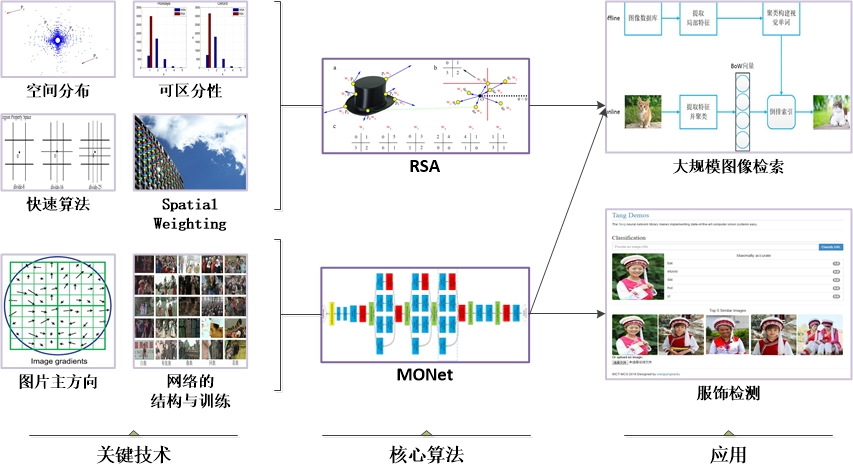
\includegraphics[width=0.9\textwidth]{frame_3.jpg}
	\caption{研究框架图}\label{fig:frame}
\end{figure}
尽管研究者们已经对图像检索中的几何校验做出了各种各样的尝试,但该领域仍然存在许多尚待解决的问题。例如如何快速的进行几何校验,同时不增加系统的负担;如何更好的解决图片旋转的问题,使几何校验算法可以更好的应用于实际的图像检索系统中去。为了解决上述问题,本文按照图\ref{fig:frame}所示的框架,提出了更加实用的几何校验方案Region Similarity Arrangement(RSA)。RSA不会增加BoW检索框架的内存,并且只需要很少的计算量,但是可以显著的提高的BoW baseline的检索精度。同时利用了CNN可以更好的理解图片语义信息这一特点,提出了Main Orientation Net(NMOet)。MONet不仅可以对基于CNN的图像检索框架提供一定的几何校验,同时可以应用于传统的BoW框架中,解决了传统几何校验方案无法处理图片旋转的问题。

\section{本章小结}
本章介绍了基于BoW和基于CNN的图像检索框架。基于BoW的图像检索已经是一种比较成熟的框架,已经存在很多经典的改进算法,本章对这些算法也进行了详细的介绍,包括查询扩充、软量化、注入技术和RootSIFT。对于BoW图像检索中的几何校验算法,本章介绍了三种经典的算法,包括两种后校验算法FSM和WGC和一种检索时算法SPM。对于以上算法,我们对其优劣进行了简单的分析和总结。另外,本章还介绍了国际上关于该课题最新的一些思路和研究趋势,这为我们未来的工作指明了方向。在本章的最后,我们提出了自己的研究框架与思路,在接下来的章节中,我们将按照该框架展开我们的研究工作。

